\documentclass{beamer}
\usepackage [russian]{babel}
\usepackage {amssymb}
\usepackage {amsmath}
%\usepackage {beamerthemeBerlin}
\usetheme{Darmstadt}
%\usetheme{Warsaw}
\title{Моделирование поведения нефтяных пятен}
\author{
	Алексей Осипов\inst{1, 2}
}
\institute{
	\inst{1}
	Синкретис
	\inst{2}
	Тинькофф
}
\date{Октябрь 2023}
\begin{document}
\begin{frame}
\titlepage
\end{frame}	
\begin{section}{Введение}
\begin{frame}{Постановка задачи}
По снимкам высокой точности необходимо предоставить возможность:
\begin{itemize}
	\item автоматически обнаруживать нефтяные пятна,
	\item прогнозировать изменение нефтяного пятна со временем,
	\item моделировать влияние на поведение нефтяного пятна различных параметров,
	\item прогнозировать прошлое поведение нефтяного пятна.
\end{itemize}

\begin{figure}[H]
	\centering
	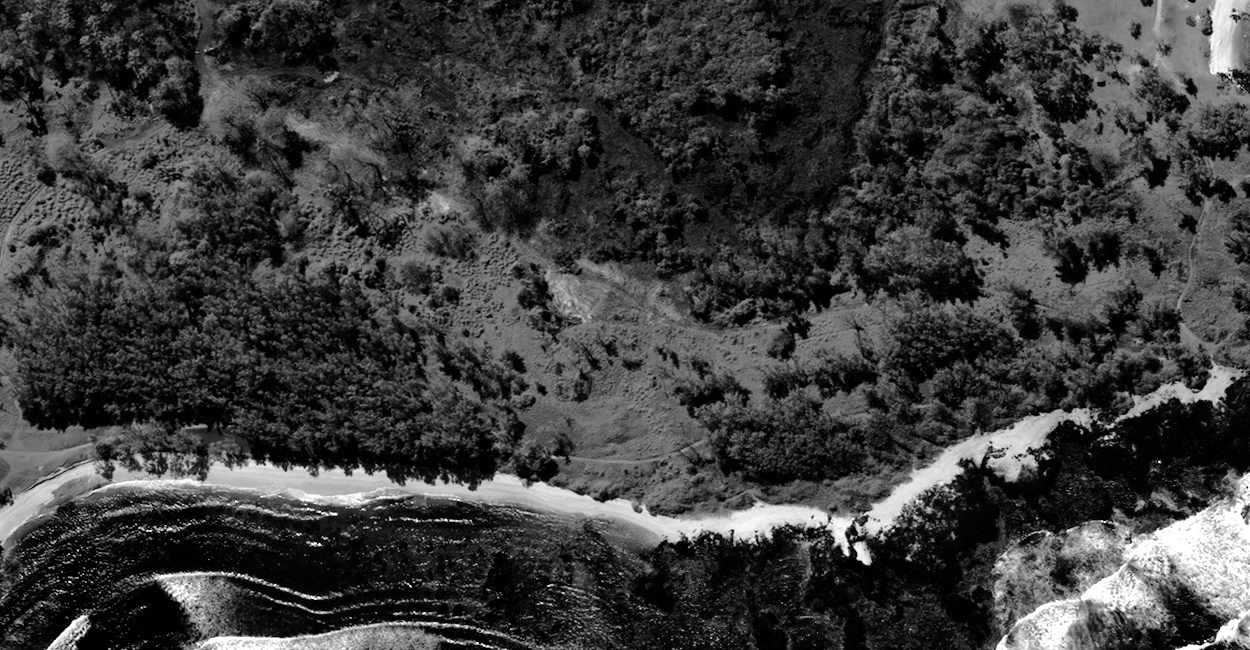
\includegraphics[scale=0.1]{maxar_8thAugust_1_21_45.png}
\end{figure}
\end{frame}
\begin{frame}{OilSync}
\begin{itemize}
	\item \textbf{OilSync} --- ПО для моделирования поведения нефтяных пятен, решающее поставленные задачи,
	\item регистрация в реестре Российского ПО, реестровая запись №19208 от 23.09.2023
\end{itemize}

\begin{figure}[H]
	\centering
	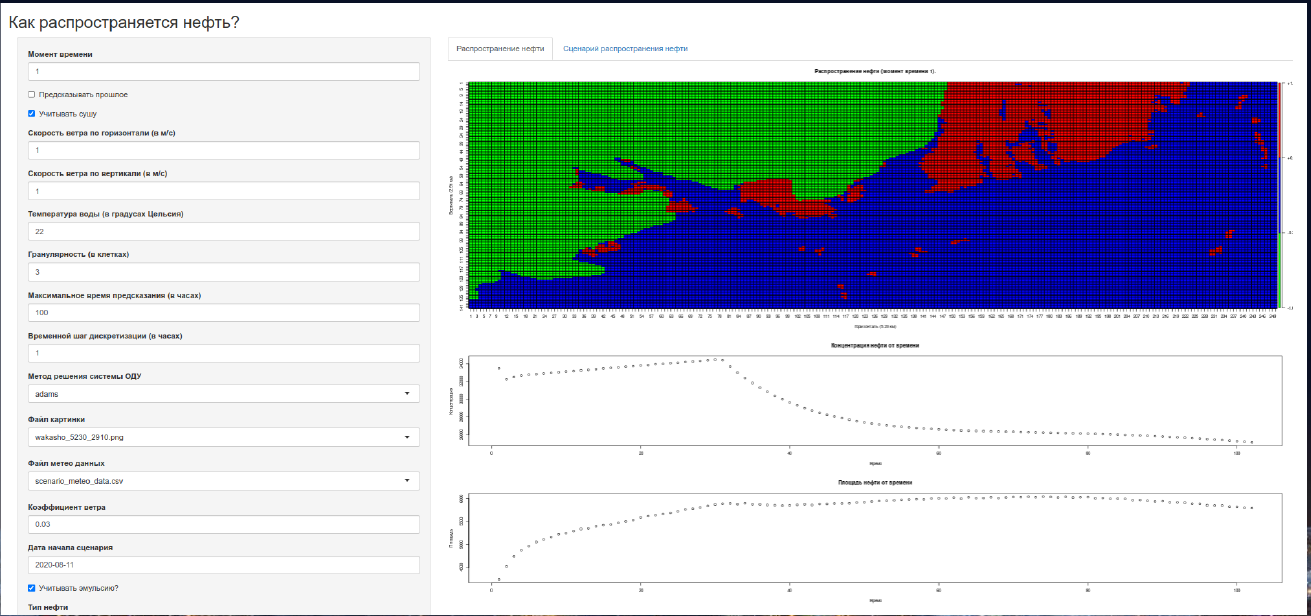
\includegraphics[scale=0.2]{how_oil_spreads.png}
\end{figure}
\end{frame}

\begin{frame}{Общая схема решения}

\begin{figure}[H]
	\centering
	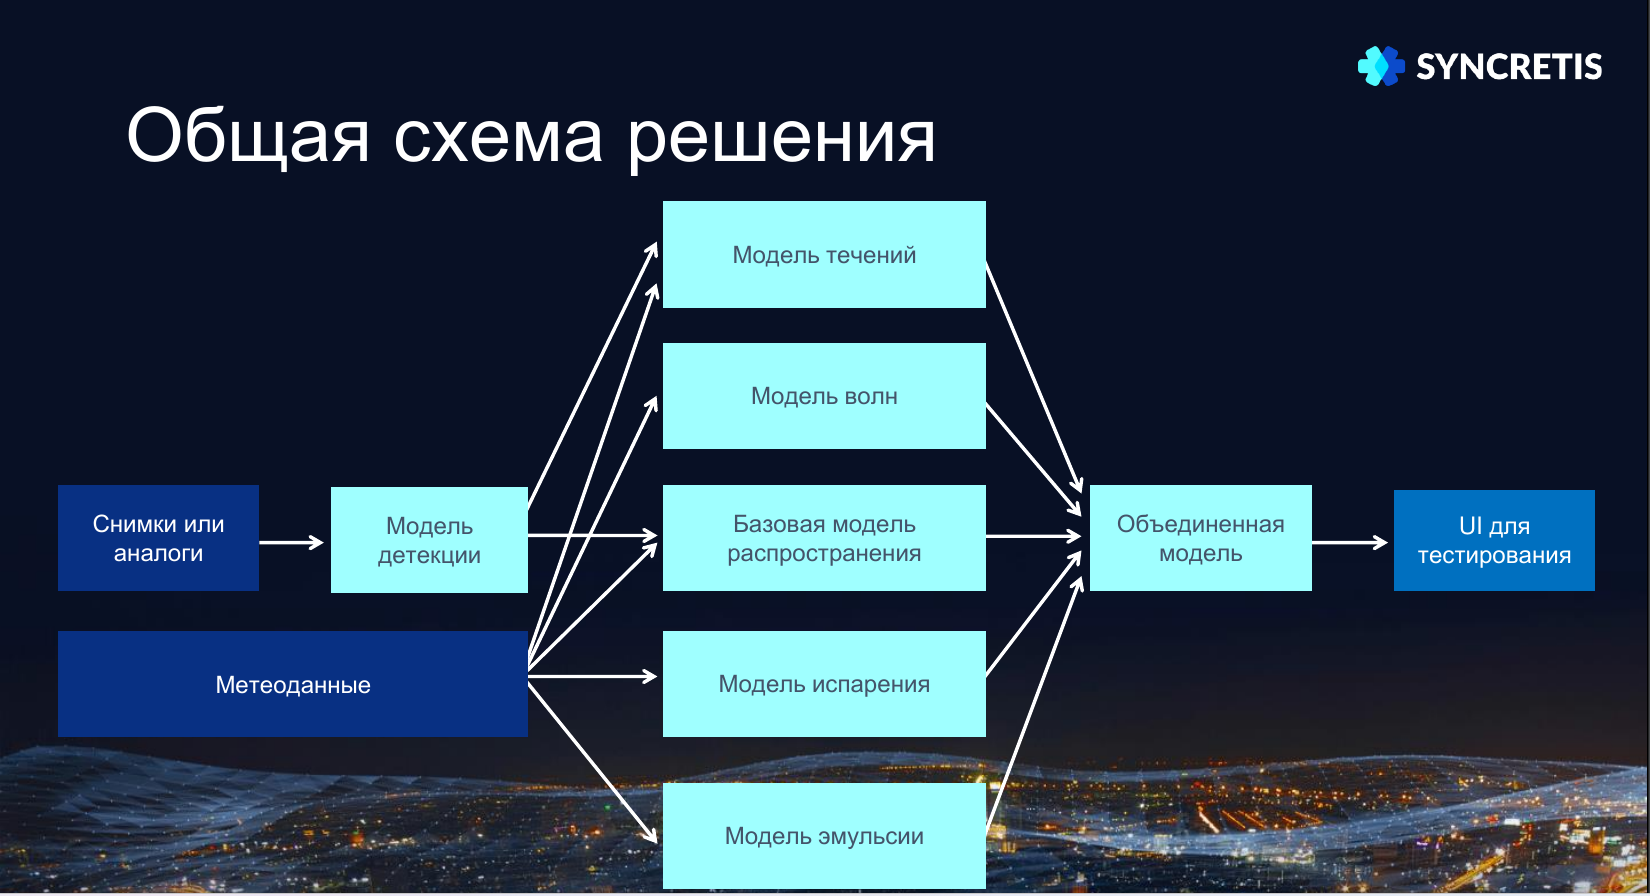
\includegraphics[scale=0.15]{general_scheme_for_oil.png}
\end{figure}
	
\end{frame}

\begin{frame}{Текущая ситуация}
		
\begin{enumerate}
	\item Задача детекции в целом решена.
	\item В задаче распространения нет хорошего решения из-за наличия большого числа факторов
	\begin{itemize}
		\item есть open-source решения (например, \textbf{gnome}, \textbf{HyosPy}), есть закрытые решения,
		\item \textbf{Эйлерова формулировка}, пятно как единое целое,
		\item Лагранжева формулировка, пятно как набор частиц.
	\end{itemize}
\end{enumerate}

\begin{figure}[H]
	\centering
	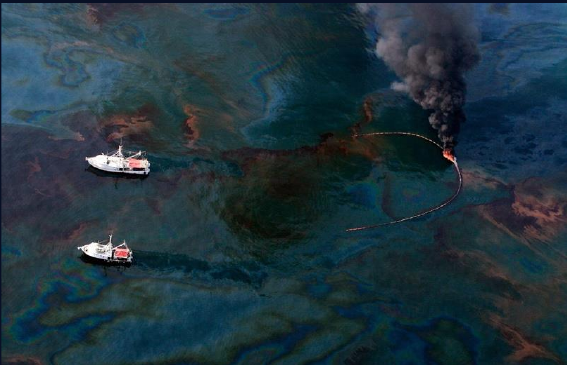
\includegraphics[scale=0.25]{example_oil.png}
\end{figure}
		
\end{frame}

\end{section}

\begin{section}{Задача детекции}
	\begin{frame}{Данные для детекции}
	\begin{itemize}
		\item Датасет для исследовательских учреждений (https://m4d.iti.gr/oil-spill-detection-dataset/)
		
		\begin{figure}[H]
			\centering
			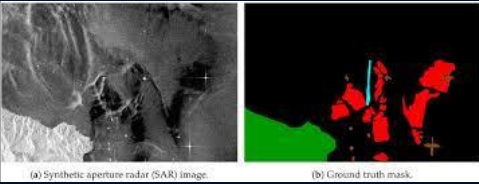
\includegraphics[scale=0.2]{greek_dataset_example.png}
		\end{figure}
		
		\item Датасет Синкретиса: weak labelling (эвристики и кластеризация на данных Maxar)
		
		\begin{figure}
			\centering
			\begin{minipage}{0.5\textwidth}
			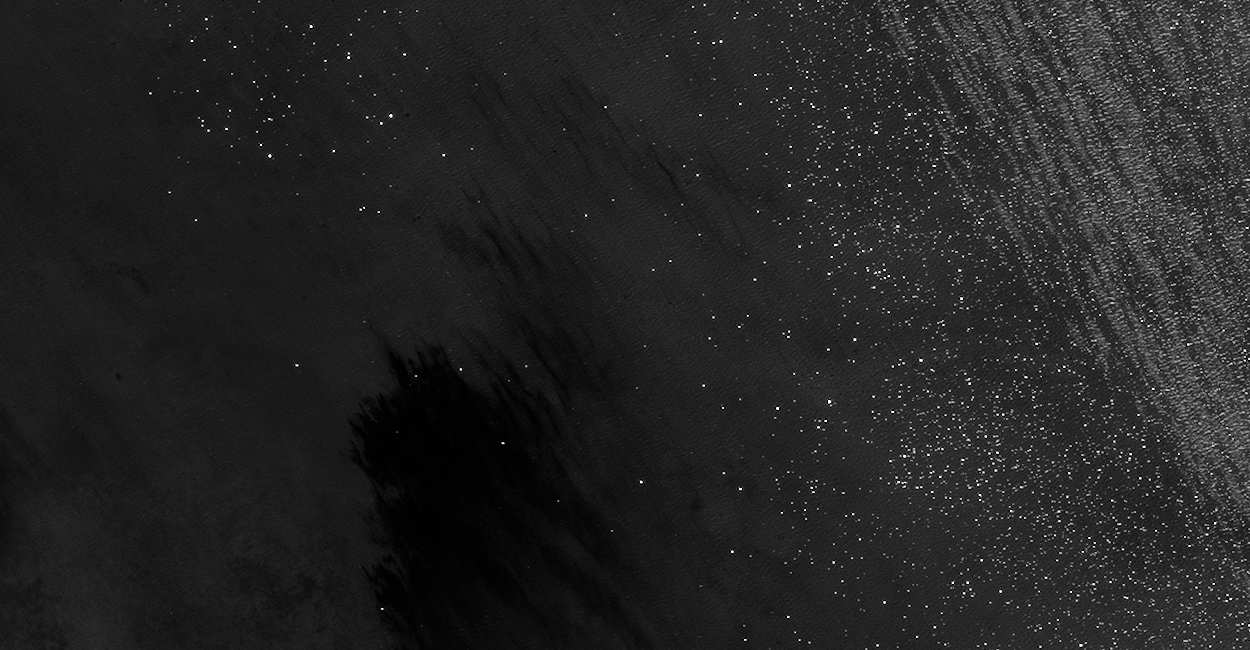
\includegraphics[scale=0.1]{maxar_8thAugust_1_26_28.png}
			\end{minipage}%
		    \begin{minipage}{0.5\textwidth}
		    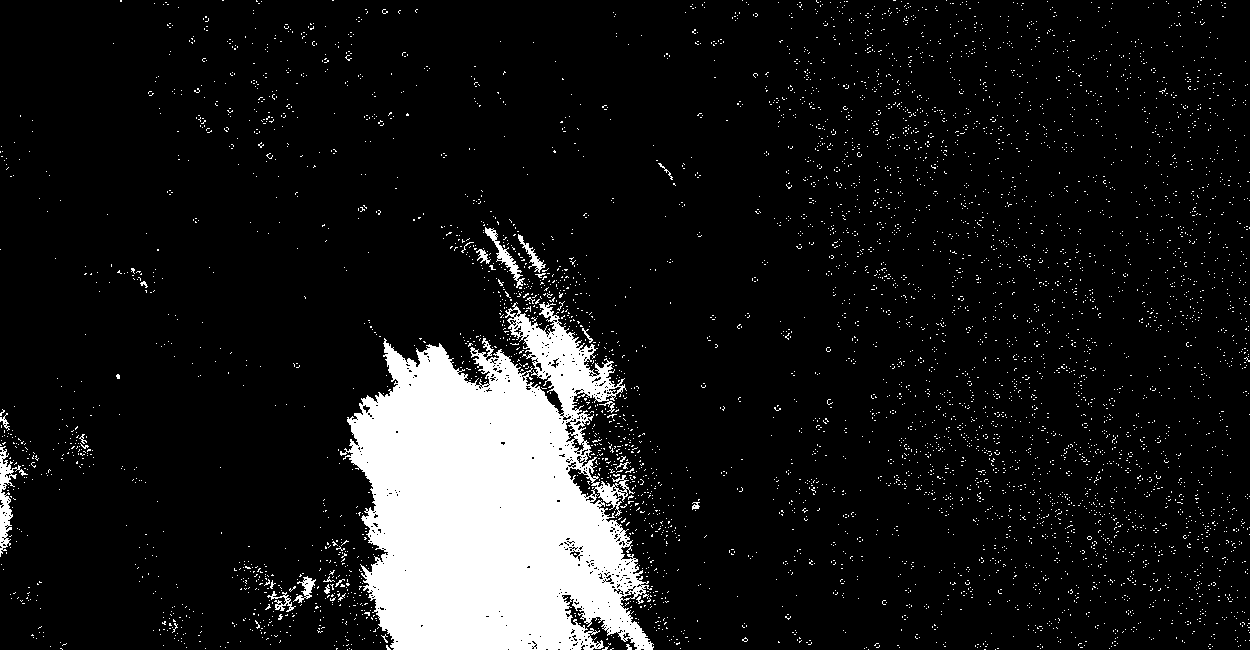
\includegraphics[scale=0.1]{maxar_8thAugust_1_26_28_mask.png}
		    \end{minipage}
	    \end{figure}
	
	\end{itemize}
	\end{frame}

\begin{frame}{DeepLabV3+}
\begin{figure}[H]
\centering
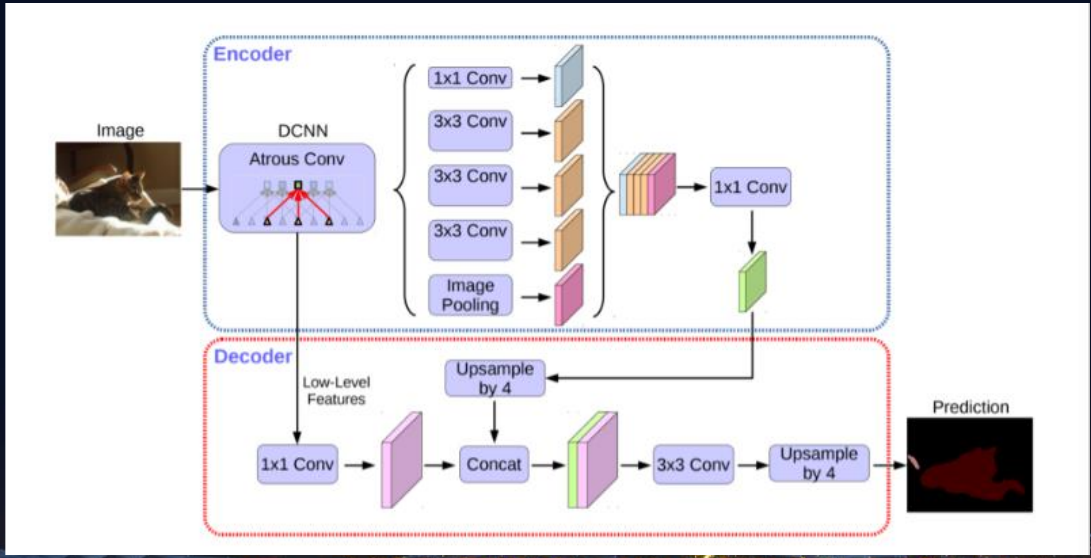
\includegraphics[scale=0.25]{deeplabv3plus.png}
\end{figure}
\end{frame}

\begin{frame}{Модель детекции}
	\begin{itemize}
		\item Лучшие модели из статей \textbf{Krestenitis et al}:
		\begin{enumerate}
			\item DeepLabV3+ с ResNet101,
			\item DeepLabV3+ с MobileNetV2,
			\item UNet.
		\end{enumerate}
	    \item Модель детекции Синкретиса:
	    DeepLabV3+ с ResNet50,
	    \item Во всех случаях mean IoU порядка 0.65
	\end{itemize}

\begin{figure}[H]
	\centering
	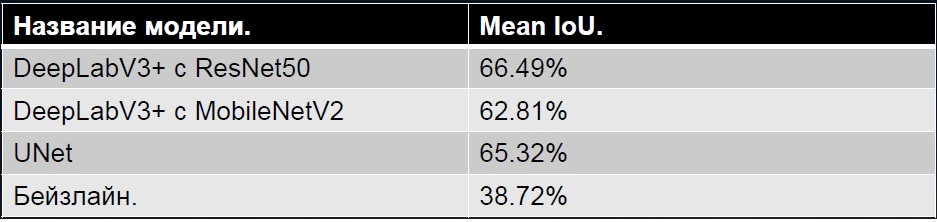
\includegraphics[scale=0.4]{table_of_syncretis_results.png}
\end{figure}

\end{frame}

\begin{frame}{Примеры результатов}
\begin{figure}[H]
	\centering
	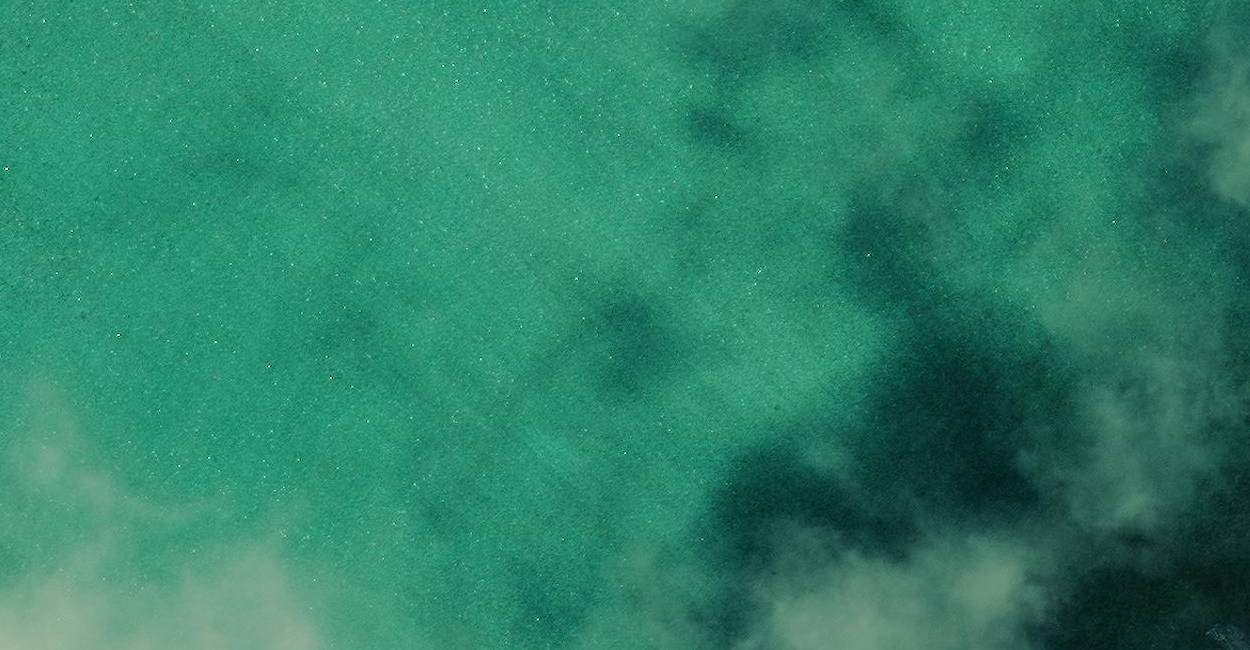
\includegraphics[scale=0.1]{maxar_maxar_16th_October_27_217_image.png}
\end{figure}

\begin{figure}
	\centering
	\begin{minipage}{0.5\textwidth}
		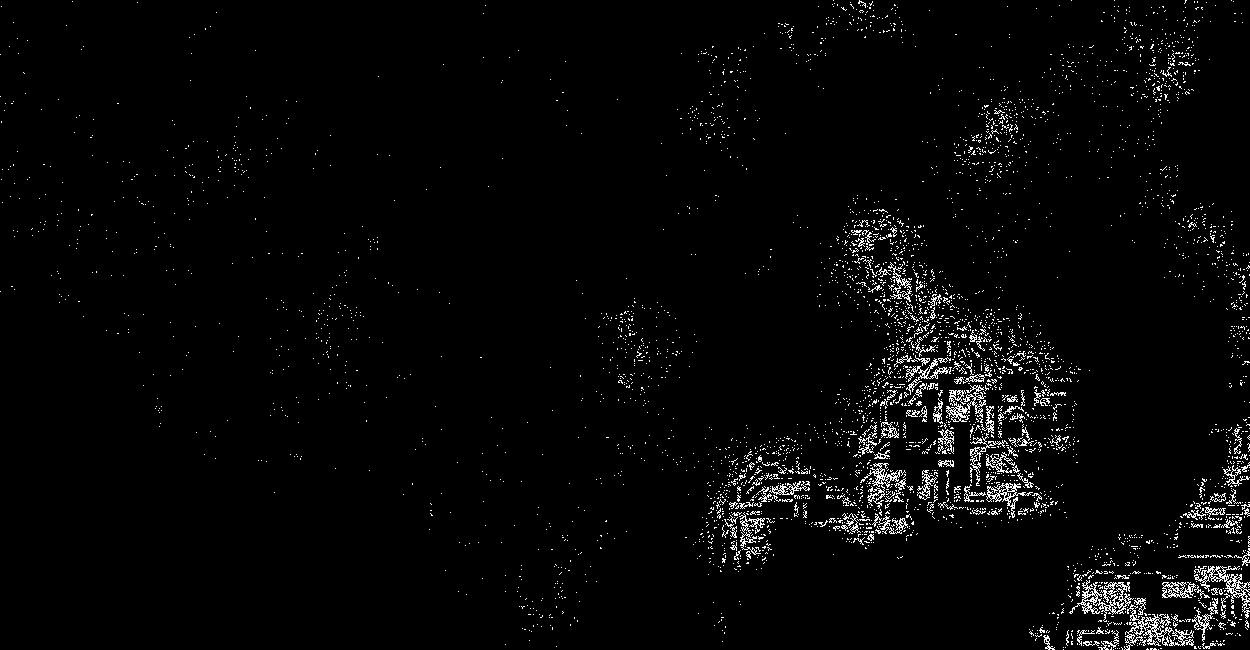
\includegraphics[scale=0.1]{maxar_maxar_16th_October_27_217_mask.png}
	\end{minipage}%
	\begin{minipage}{0.5\textwidth}
		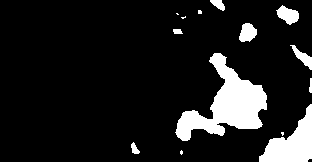
\includegraphics[scale=0.4]{maxar_maxar_16th_October_27_217_results.png}
	\end{minipage}
\end{figure}

\end{frame}

\end{section}
\begin{section}{Модель распространения}
\begin{frame}{Входные данные}
\begin{itemize}
\item Скорость ветра (вектор).
\item Температура воды (для коэффициента диффузии).
\item Данные о пятне и о суше.
\item Данные о времени.
\end{itemize}
Динамическая система.

\begin{figure}
	\centering
	\begin{minipage}{0.5\textwidth}
		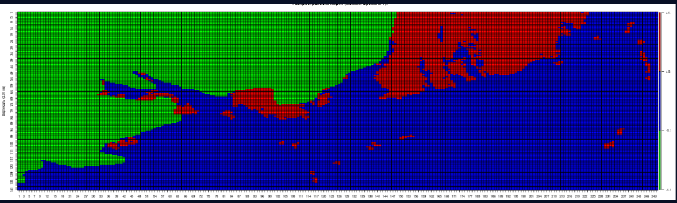
\includegraphics[scale=0.2]{photo_before.png}
	\end{minipage}%
	\begin{minipage}{0.5\textwidth}
		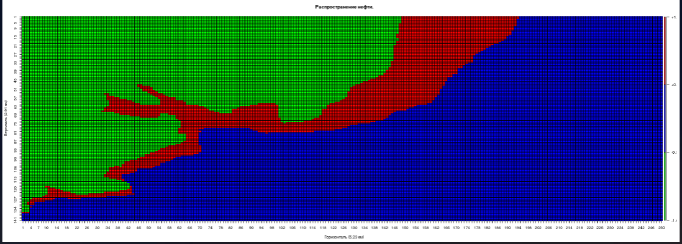
\includegraphics[scale=0.2]{photo_after.png}
	\end{minipage}
\end{figure}

\end{frame}		
\begin{frame}{Входные данные}
\begin{itemize}
	\item Уравнение адвекции-диффузии на концентрацию:
	
	$$\frac{\partial C}{\partial t} + u\cdot\nabla C = \nabla (k\nabla C),$$
	$$k = 0.002\left(\frac{T}{22}\right)^{1.53}.$$
	
	\item Граничные условия соответствуют обнаруженному пятну.
	
	\item Дискретизация и сведение к системе ОДУ.
	
	\item Решения системы ОДУ методом Адамса.
	
	\item Модель взята из работы \textbf{Duran et al}.
	
\end{itemize}
\end{frame}

\begin{frame}{Особенности базовой модели}
\begin{itemize}
	\item Скорость ветра может зависеть от времени и от координаты.
	\item Учет суши проводится отдельным скриптом.
	\item Обратная задачи у модели не разрешима, у приближения разрешима. 
\end{itemize}

\begin{figure}[H]
	\centering
	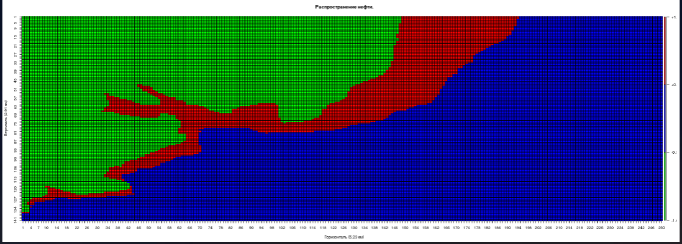
\includegraphics[scale=0.2]{photo_after.png}
\end{figure}
\end{frame}

\begin{frame}{Данные модели течений}
\begin{itemize}
	\item Данные о течениях \textbf{Woods Hole Oceanographic Institution}.
	\item Короткие временные ряды.
	\item Завиимость от географических координат.
	\item Годовая нарезка данных.
\end{itemize}

\begin{figure}[H]
	\centering
	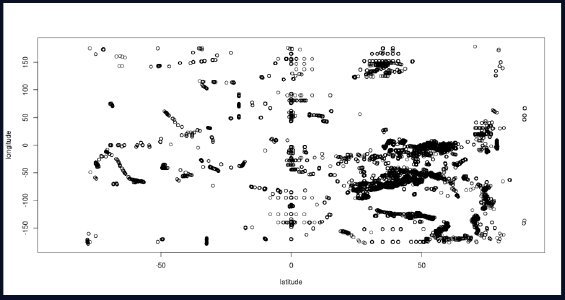
\includegraphics[scale=0.3]{scatter_plots_on_currents.png}
\end{figure}
\end{frame}

\begin{frame}{Прогноз модели течений}
\begin{itemize}
	\item Компоненты решения: эвристики, HDBSCAN, SMA, EMA, Catboost, VAR.
	\item Модель: блендинг модели, основывающейся на HDBSCAN, EMA, VAR.
	\item MAPE порядка 0.45.
	\item Приближение точки усреднением по кластеру при прогнозировании.
\end{itemize}

\begin{figure}[H]
	\centering
	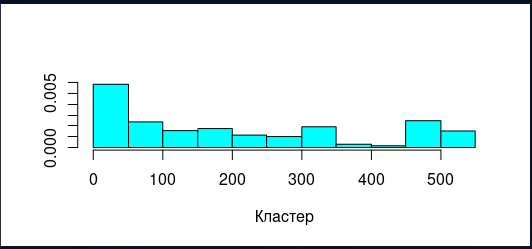
\includegraphics[scale=0.3]{histogram_on_currents.png}
\end{figure}

\end{frame}

\begin{frame}{Выбор модели для течений}

\begin{figure}[H]
	\centering
	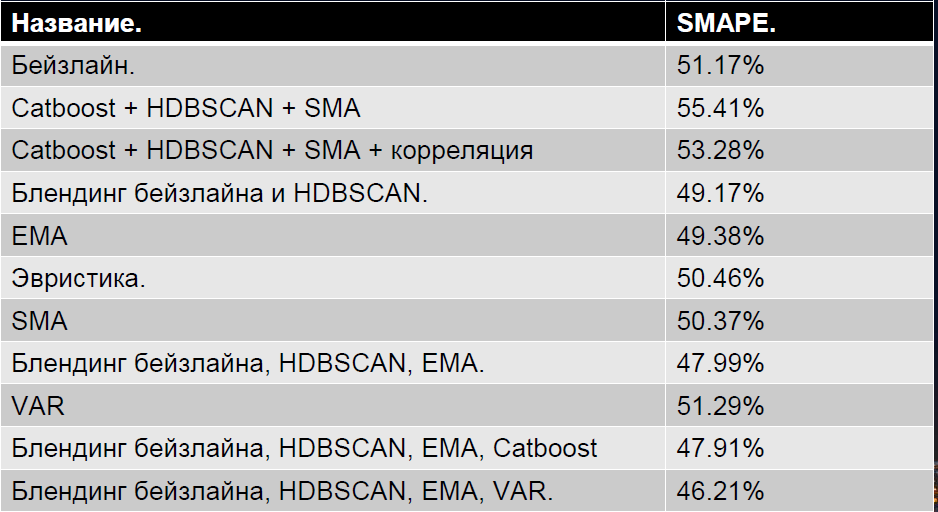
\includegraphics[scale=0.55]{currents_choice_of_model.png}
\end{figure}

\end{frame}

\begin{frame}{Модель волн}
\begin{itemize}
	\item Модель Sverdrup, Munk, Bretschneider.
	\item Эмпирическая модель, основанная на скорости ветра и fetch length:
	$$H = 0.283\alpha \frac{W^2}{g}\tanh\left(\frac{0.0125}{\alpha}\left(\frac{gF}{W^2}\right)^{0.42}\right),$$
	$$T = 7.54\beta\frac{W}{g}\tanh\left(\frac{0.077}{\beta}\left(\frac{gF}{W^2}\right)^{0.25}\right),$$
	$$\alpha = \tanh\left(0.53 \left(\frac{gH}{W^2}\right)^{0.75}\right),\quad \beta = \tanh\left(0.833\left(\frac{gH}{W^2}\right)^{0.375}\right),$$
	где $H$ --- высота волны, $T$ --- период волны, $W$ --- скорость ветра, $F$ --- fetch length.
\end{itemize}
\end{frame}

\begin{frame}{Модель испарения}
Модель из работы Fingas:
$$E = KCU^{7/9}d^{-1/9}\textrm{Sc}^{-r},$$
\begin{itemize}
	\item $K$ --- коэффициент переноса массы,
	\item $C$ --- концентрация нефти,
	\item $U$ --- скорость ветра,
	\item $d$ --- площадь поверхности водоема,
	\item Sc --- число Шмидта,
	\item $r$ --- эмпирическая константа. 
\end{itemize}
\end{frame}

\begin{frame}{Модель эмульсификации}
Под эмульсификацией подразумевается смешивание воды и нефти.

Модель из работы Aghajanloo et al:
$$\frac{\partial D}{\partial t} = K \left(1 + U\right)^2\left(\frac{1 - F}{OC}\right),$$
\begin{itemize}
	\item $K$ --- коэффициент эмульсификации, 
	\item $U$ --- скорость ветра,
	\item $OC$ --- константа, характеризующая тип нефти.
\end{itemize}
\end{frame}

\begin{frame}{Модель вертикального транспорта}
\begin{itemize}
	\item Нефть погружается на дно, а потом всплывает.
	\item Трехмерное обобщение базовой модели.
	\item Модель взята из работы Aghajanloo et al.
	\item Проблема с начальными условиями.
\end{itemize}

$$\frac{\partial C}{\partial t} + \frac{\partial u C}{\partial x} + \frac{\partial v C}{\partial y} - \frac{\partial w C}{\partial z} = \frac{\partial}{\partial x}D_x\frac{\partial C}{\partial x} + \frac{\partial}{\partial y}D_y\frac{\partial C}{\partial y} + \frac{\partial}{\partial z}D_z\frac{\partial C}{\partial z},$$

где $C$ --- концентрация, $u$, $v$ --- скорости, $w$ --- скорость всплывания, $D_x$, $D_y$, $D_z$ --- коэффициенты диффузии.
\end{frame}

\end{section}

\begin{section}{Заключение}

\begin{frame}{Особенности}
	\begin{itemize}
		\item Наличие индивидуального режима работы и режима сценария с возможностью валидации на исторических событиях.
		\item Присутствуют модели и детекции, и распространения.
		\item Модель достаточно сложна и достаточно гибка, в нее можно включать дополнительные факторы.
		\item Эйлерова формулировка в модели распространения в отличие от формулировки Лагранжа в большинстве других решений.		
	\end{itemize}
\end{frame}

\end{section}

\begin{frame}{Спасибо за внимание!}

\begin{block}{Мои контакты}
\begin{itemize}
	\item мой e-mail: osipovav28@googlemail.com
	\item моя личная страничка: https://sites.google.com/site/osipovav39/
	\item репозитории: https://github.com/AlexO28
\end{itemize}
\end{block}
\begin{block}{контакты компании Синкретис}
\begin{itemize}
	\item e-mail компании Синкретис: info@syncretis.ru,
	\item сайт компании Синкретис: https://syncretis.com/ru
\end{itemize}
\end{block}

\end{frame}

\end{document}
